% sections/results.tex — PROSE + references to GENERATED files.
%
% The prose here is safe to live-edit on Overleaf. The figures
% (../figures/*.png) and the model table (output/tabs/model_table.tex) are
% produced by R/03_analysis.R and pushed — do NOT hand-edit those; re-run
% the script and they update on the next compile.
\section{Results}

\subsection{Main effect}

\begin{figure}[h]
  \centering
  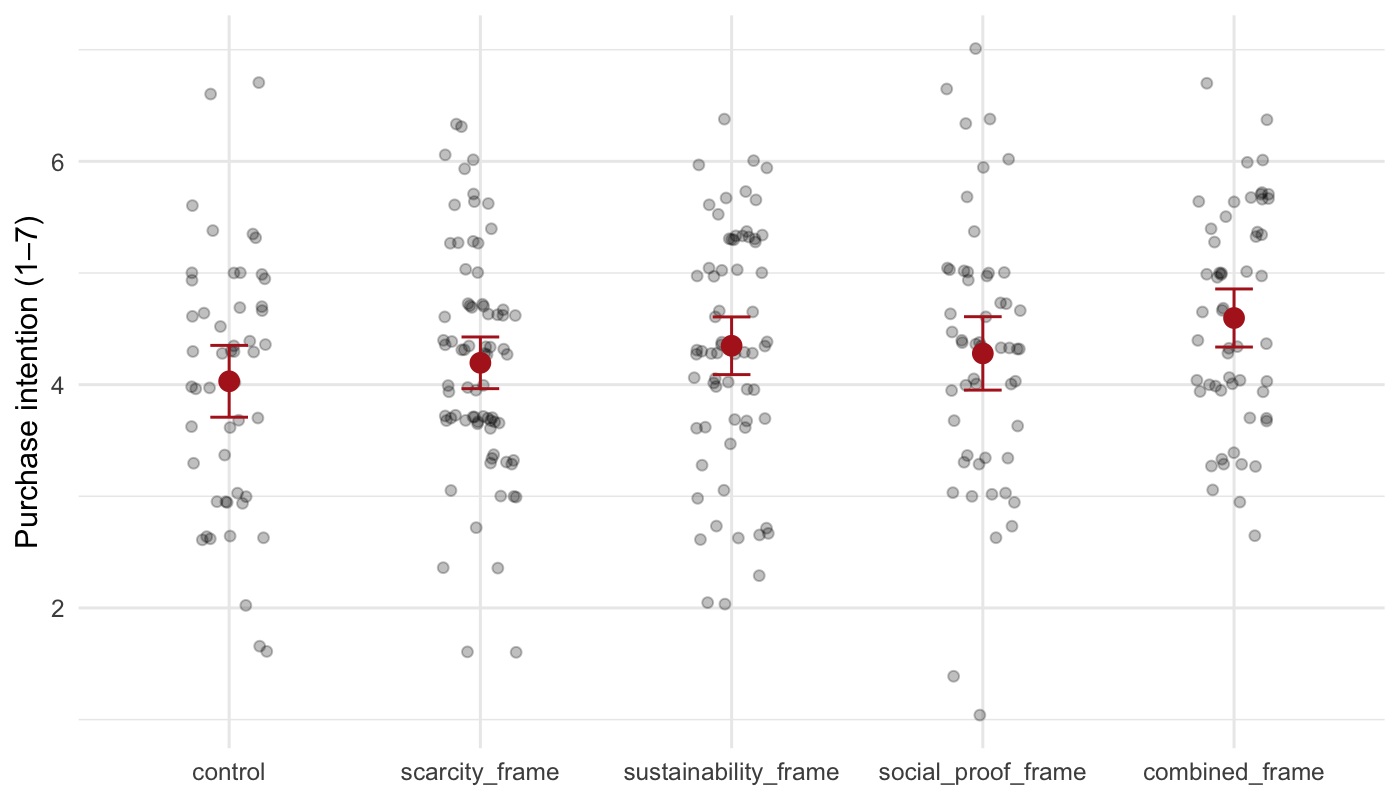
\includegraphics[width=0.85\textwidth]{../figures/fig_01_pi_by_condition.png}
  \caption{Purchase intention by condition. Red points are condition means
           with 95\% confidence intervals.}
  \label{fig:main}
\end{figure}

\subsection{Mediation through perceived value}

\begin{figure}[h]
  \centering
  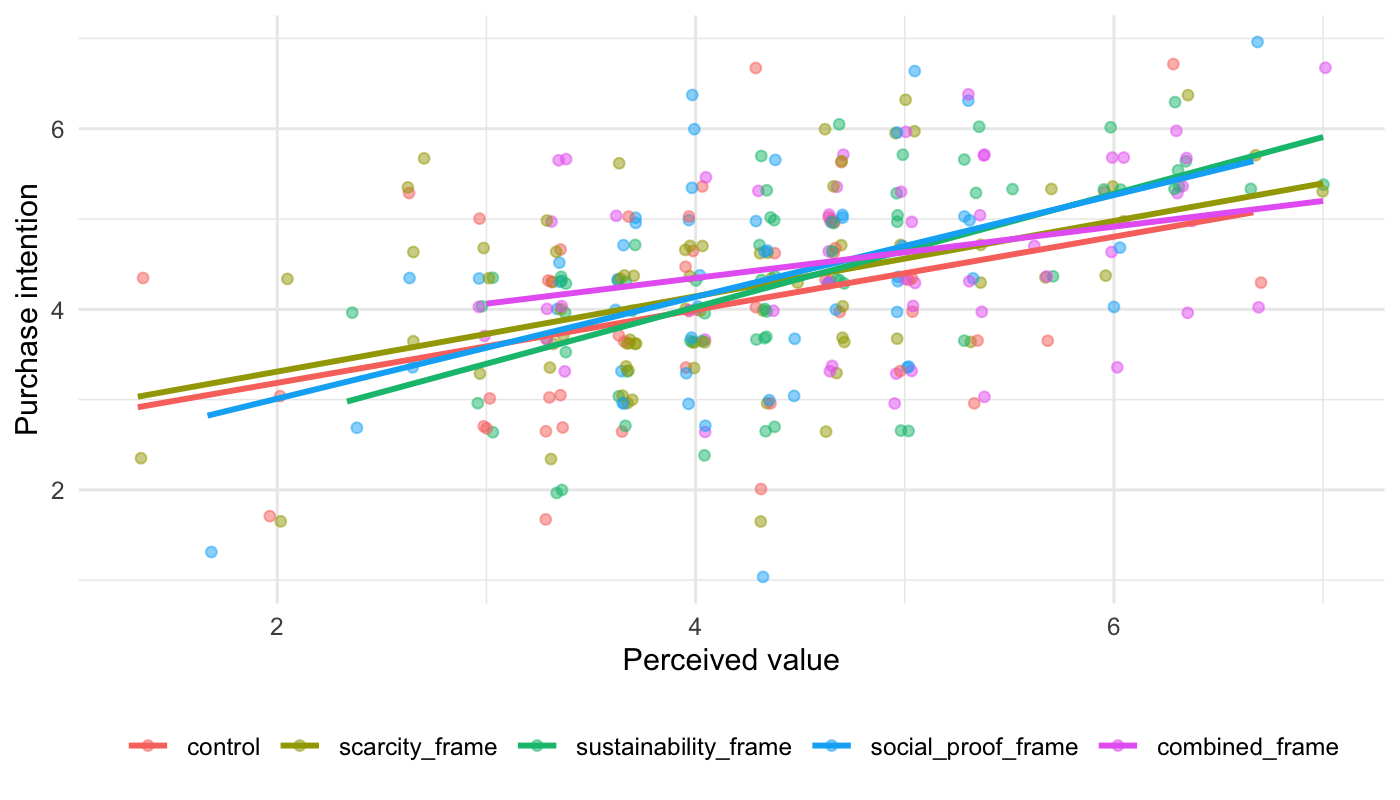
\includegraphics[width=0.85\textwidth]{../figures/fig_02_mediation_scatter.png}
  \caption{Perceived value predicts purchase intention; the conditions
           shift perceived value upward, producing an indirect path.}
  \label{fig:mediation}
\end{figure}

\subsection{Moderation by price sensitivity}

\begin{figure}[h]
  \centering
  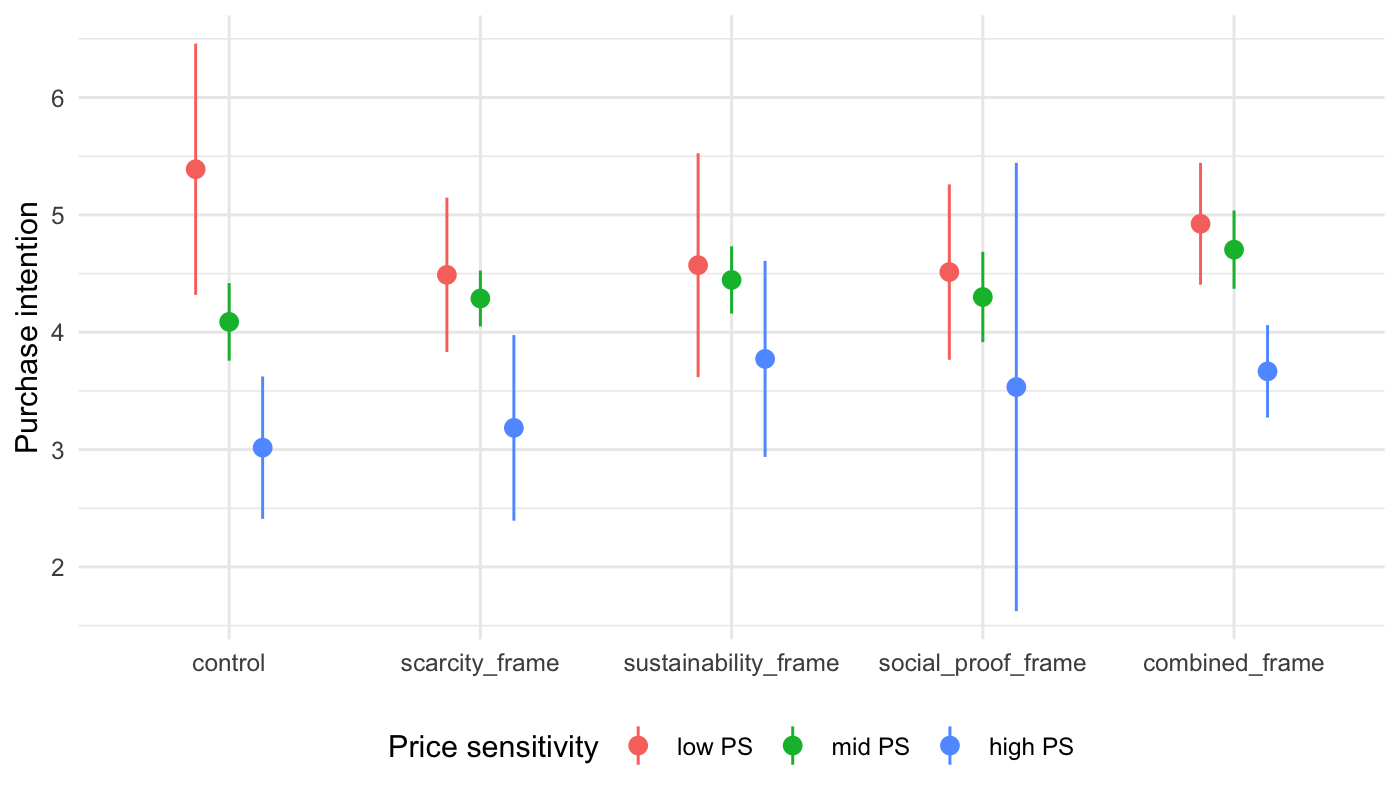
\includegraphics[width=0.85\textwidth]{../figures/fig_03_moderation.png}
  \caption{The condition boost is attenuated for high-price-sensitive
           respondents.}
  \label{fig:moderation}
\end{figure}

\subsection{Model estimates}

Table~\ref{tab:models} collects the coefficients behind the figures above.
It is generated by \texttt{R/03\_analysis.R} and written straight into
\texttt{output/tabs/}, so the numbers in the paper can never drift from the
numbers in the analysis.

\input{output/tabs/model_table.tex}
